\section{MIP Formulation} \label{mip}

\subsection{Mix Integer Programming}
Mix Integer Programming (MIP) is a common optimization technique that is widely used by the research community to study weakly hard models. An optimization problem is called an integer programming problem if its decision variables are constrained to integer values. MIP is a special form of integer programming problem in that some variables, but not all, are constrained to be integers. A common type of decision variables in MIP is binary variable whose value is restricted to be 0 or 1, which formulates yes/no question. However, integer programming is NP-Hard because it is not convex, so it takes a large amount of computation time and memory resources to find an optimal solution. In spite of the complexity, industrial solvers can solve small size MIP problem relatively fast. 

\subsection{Ethernet-based Switch Network}
This section considers the application-level scheduling problem on a time-triggered, Ethernet based distributed system ~\cite{Zhang2018SynthesizingCA}. Specifically, a switch network is considered. This network can be model as an undirected graph. The nodes of the graph are end stations and switches that forward messages between end stations. An edge between two nodes represents a full-duplex link that allows simultaneous message transmissions between two nodes. An example of this graph-based presentation of a Ethernet-based switch network is shown in Figure ~\ref{fig:network}.

\begin{figure}[h!]
\caption{A model of Ethernet-based Switch Network~\cite{Zhang2018SynthesizingCA}}
\centering
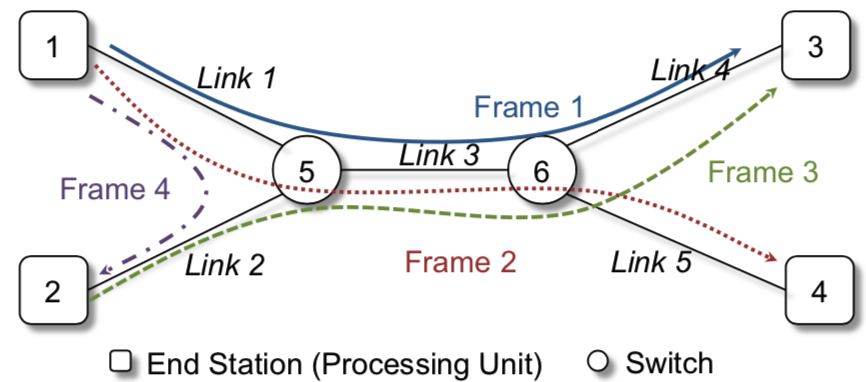
\includegraphics[width=0.5\textwidth]{network}
\label{fig:network}
\end{figure}

\subsection{MIP Formulation}
Zhang ~\cite{Zhang2018SynthesizingCA} formulates the application-level scheduling problem on a time-trigger, Ethernet-based switch network as an MIP problem. The tasks to be scheduled on the distributed system can be classified into application tasks that run on the end stations and communication tasks that should be scheduled on the Ethernet network. 

The first constraint on the MIP program formulation requires that application tasks are collision-free. The assumption for the distributed system is that each end station only consists of a single processor, so this constraint ensures that only one application task can be run on any end station at any given time stamp. The second constraint ensures that communication tasks are collision-free as well. At most one communication task can be transmitted on one direction of any link at any time stamp. 

Path dependency and data dependency are formulated as constraints as well. Path dependency for a communication task is formulated such that each frame has to be forwarded in the correct temporal order defined by its path to ensure that the message reaches the correct end station. Data dependency in application tasks requires application tasks and their corresponding communication tasks to be schedule in the correct temporal order. 

Constraints on response time and end-to-end latency on application tasks have also been exploited. Both the response time and the end-to-end latency are formulated as hard constraints, but adopting weakly hard constraints can provide looser constraints on response time, thus expanding the scope of schedulable task sets. Future work can be done on this direction.

Zhang ~\cite{Zhang2018SynthesizingCA} considered multiple objectives in this problem formulation. These objectives include response time and end-to-end latency in the average case and in the worst case, as well as certain timing requirements on specific tasks. The objective function, as a result, is a sum of each weighted sub-objective.


